\chapter{Lung Cancer, Radiotherapy and Computed Tomography}\label{ch:soa}

\section{Lung Cancer and treatment}


Lung cancer is the most common cancer in the world in men, both in amount of cases and mortality. In women, is third in cases and second in mortality, after breast cancer\cite{WCR2014}. Yearly deaths due to lung cancer go over 1.5 million (see figure \ref{fig:world} for incidence), having around 10\% of five year survival rate in developed countries, and much lower in developing countries\cite{CRUK2014}. One over fourteen people has a lifetime risk of developing lung cancer\cite{Harrisons2012}, in average between men and women. The high incidence and mortality rates has lead to a big amount of research in research fields from all disciplines, in order to push further the detection and treatment of the disease, with an output of over 23.000 lung cancer related research articles in prestigious journals in the last 10 years\cite{Nature2015}. In addition, the  actual lung cancer treatment has been transformed from non-existent in the 70s to used worldwide\cite{Comis2003}.


\begin{figure}[ht]
\begin{center}
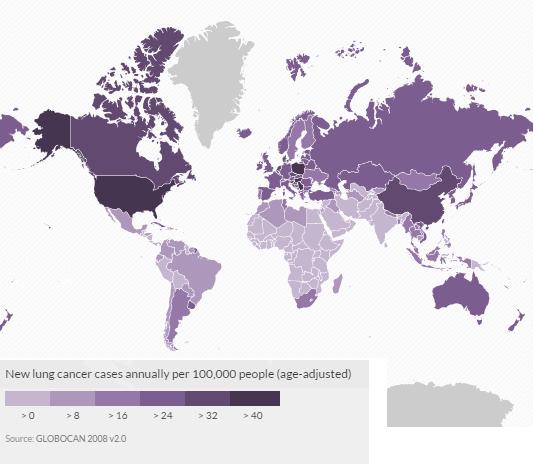
\includegraphics[width=0.98\columnwidth]{StateOfArt/worldmap.png}
\caption[Lung cancer incidence in the world]{Lung cancer incidence per country, age adjusted data. Map and data from {GLOBOCAN}\cite{GLOBOCAN2010}.}
%IARC has proprietary rights to the materials on the Website. Publications/data made available by IARC/WHO enjoy copyright protection in accordance with the provisions of Protocol 2 of the Universal Copyright Convention. All rights are reserved. Materials (fact sheets, maps, estimates or data) may be used "as is" for research, educational or other non-commercial purposes, but the corresponding reference must be cited in all cases.
\label{fig:world}
\end{center}
\end{figure}



The treatment of lung cancer varies between different types, but there are four main techniques: Chemotherapy, lobectomy or pneumoctomy, radiotherapy (RT) and palliative care. Generally, in early stages of small cell lung cancer the typical treatment would consist in chemotherapy with radiotherapy, and then brain radiotherapy, as there is chance that the tumour would spread to the head when treated. If the tumour has been detected in a very early stage and has not spread to the lymph nodes a lobectomy may be performed, removing part of the lung. Usually this is followed by radiotherapy and chemotherapy to make sure the tumour is killed.
In the case of non-small cell lung cancer, in the first stages a lobectomy or a pneumoctomy (removal of the whole lung) may be performed. Generally radiotherapy and chemotherapy (less likely) are also performed. In the last stages of the cancer, usually the treatment is palliative care i.e. treatments to reduce the symptoms and relief pain\cite{CRUK2014b}.

In practically all stages of different lung cancer treatments, radiotherapy is extensively used. About 120.000 patients use radiotherapy in the UK every year. Radiotherapy aims to kill malignant cells using ionizing radiation, generally using photons. High energy photons (X-rays) ionize the atoms that are part of the DNA chain. In photon therapy, this happens due to the ionization of the water in the cells, that forms free radicals, such as hydroxil radicals, destroying the DNA of the cells and killing them.

\section{Image Guided Radiation Therapy}

\section{Motion in CBCT}
Due to the lower doses used than in a conventional CT scan and to its slow data acquisition rate, a CBCT image is generally riddled with noise and motion artefacts.  Research into the removal of motion artefacts in CBCT is widespread and numerous articles have been published on the subject.  The most studied method to deal with motion is phase-correlated CBCT, also called 4D-CBCT\cite{sonke2005respiratory}\cite{thomas2006}\cite{li2006four}\cite{Pengpan2012246}\cite{t2016first}.  In 4D-CBCT, projection data are binned according to respiratory phase and then the data from each bin are reconstructed separately to produce a series of images.  This approach has several drawbacks.  Even though the amount of data per reconstructed image is smaller than usual, the total number of projections increases which means a longer irradiation time and a higher dose for the patient, limiting its clinical use.  In addition, the image quality of each 4D-CBCT reconstruction is inferior to a 3D-CBCT one due to its reduced angular sampling and to small inconsistencies resulting from binning inaccuracies. 

Due to the limitations of standard 4D-CBCT imaging, extensive research has been conducted to improve the quality of the images.  This work can be divided into two main groups: algorithmic approaches and deformation vector field (DVF) optimization methods.  Methods in the first group rely on regularization and other similar approaches.  An example is the work by Jia \textit{et al.}\cite{jia2012}, who implemented a non-local means of reconstruction to improve the temporal similarity between images.  Total variation methods (TV)\cite{ASD_POCS}, which minimize gradients within an image, have been also proposed with a temporal dimension included in the gradient\cite{0031-9155-57-6-1517}.  Another method based on TV minimization is the so-called PICCS algorithm\cite{chen2008prior}\cite{0031-9155-53-20-006}\cite{chen2012time}, which minimizes the TV and the difference between the reconstructed image and a prior image.  This prior image is generally a CBCT reconstructed with motion artefacts.  PICCS can reconstruct 4D-CBCT images from highly undersampled datasets.  More complex algorithms have also been proposed, such as ROOSTER\cite{:/content/aapm/journal/medphys/41/2/10.1118/1.4860215}, where a series of regularizations and minimizations are performed inside a region of interest to create clear 4D images in that area.

The methods of the second group generally (but not always) rely on a previous high-quality 4D-CT treatment planning scan as the basis from which to compute the DVFs.  As breathing motion is neither truly periodic nor reproducible in a given patient over time, the DVFs are corrected by matching real projections with simulated ones.  Finally, when the best DVF is computed, a synthetic image is generated by deforming the prior high-quality CT scan.  Examples include the work of Brock \textit{et al.}\cite{brock2010} and Ren \textit{et al.}\cite{Ren20121584}, who managed to reduce the number of projections required to about 60 using non-linear conjugate-gradient methods.  In order to improve robustness and reduce the dimensionality of the problem, DVF principal component analysis methods have also been proposed\cite{zhang2010correction}.  Li \textit{et al.}\cite{:/content/aapm/journal/medphys/37/6/10.1118/1.3426002}\cite{:/content/aapm/journal/medphys/38/5/10.1118/1.3582693} demonstrated that good accuracy can be achieved using only a single projection for the DVF optimization.

Hybrids between DVF-based and algorithmic approaches also exist, such as using TV regularization methods to improve convergence by initializing the DVFs\cite{wang2012high} or using temporal regularization with DVFs to improve the ROOSTER algorithm\cite{mory2016motion}.  Hybrid methods can lead to highly complex optimization strategies.  Examples include segmented mesh-based 4D-CBCT\cite{0031-9155-61-3-996} and the separation of static and moving images using TV, tight frame regularization and DVF optimization\cite{0031-9155-56-11-002}.  In addition, Christoffersen \textit{et al.}\cite{christoffersen2013registration} have proposed a multi-step algorithm using TV and optical flow for motion estimation.

Finally, some special mathematical algorithms have also been suggested that are unique in their approach.  These include the cine-CBCT algorithm\cite{6803058} and the 5D motion modelling approach\cite{0266-5611-31-11-115007}, which does not use phase-correlated binning.

The literature is full of these and many other approaches, ranging from the computationally and mathematically complex to those that sacrifice accuracy for simplicity and speed.  Most have been shown to yield good 4D-CBCT reconstructions, some in clinical scenarios.  But they all have drawbacks.  CBCT is a severely ill-posed problem where the amount of data is key for a good reconstruction.  The simplest methods that rely on binning will always suffer to some extent from a lack of data, even if temporal coherence is enforced with mathematical norms.  Additionally, they involve the reconstruction of several images, which is very expensive both computationally and in terms of memory.

Most DVF-based approaches ultimately use the DVFs to deform a prior image rather than using the acquired data directly to produce a reconstruction.  Further, they assume that a DVF can describe every possible anatomical change with respect to that prior image and this does not necessarily hold.

%{red}{\sout{Here, we propose a completely different approach to motion compensation in 4D-CT imaging.}}
In this work, a modelling method for motion compensation is presented, as first proposed by Hancock \textit{et al.}\cite{pst1} outside the medical domain and later independently proposed by Rit \textit{et al.}\cite{Rit1}\cite{Rit2} for CBCT. Since the publication of their work, computing on graphical processing units (GPUs) has taken a significant leap forward affording more modern techniques that can be used to reconstruct with greater accuracy and computational efficiency. With the use of GPUs even generic motion compensation is possible, without any numerical approximation of the weights in the projection and back projection and using better forward modelling\cite{fwdproj}. Such an approach is presented in this work.

This thesis focuses on thorax CBCT, but the method is generalizable to any X-ray absorption CT modality and to arbitrary motion.  The method requires no binning, but instead uses all projections to reconstruct an image at any respiratory phase.  It does require a sufficiently accurate description of the motion in terms of DVFs, but the approach is a modelling one so it can be used to introduce motion compensation into any iterative reconstruction algorithm. 
